\documentclass[margin=2cm]{standalone}

\usepackage[dvipsnames]{xcolor}
\usepackage{tikz}
\usetikzlibrary{arrows, positioning, calc, decorations.pathreplacing}

\begin{document}
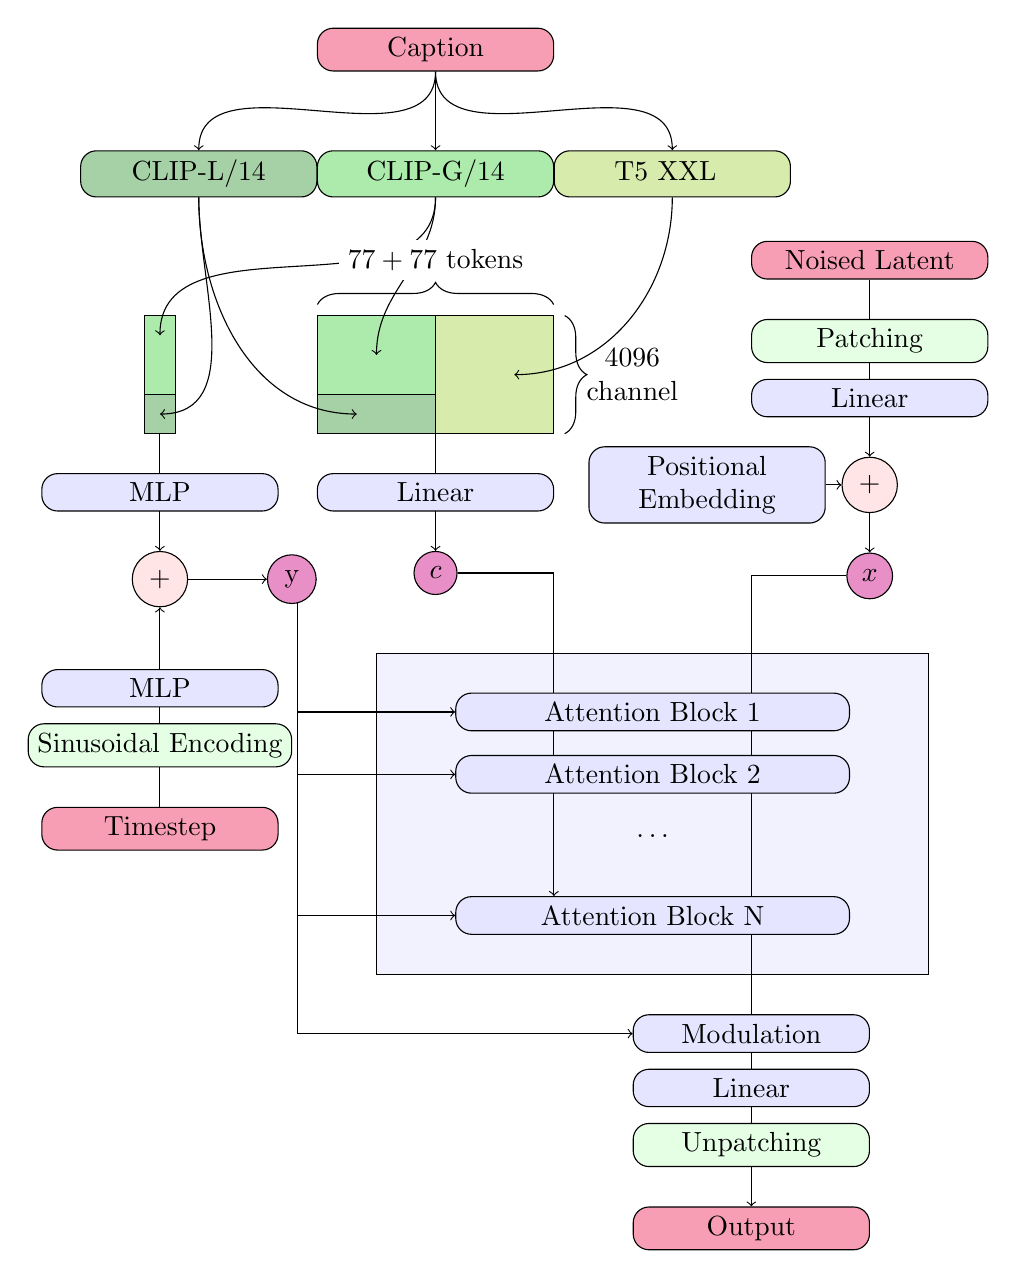
\begin{tikzpicture}[
        block/.style={draw, fill=white, rectangle, minimum width=3cm,rounded corners=0.2cm},
        trainableblock/.style={block,fill=blue!10},
        frozenblock/.style={block,fill=blue!10},
        fnblock/.style={block,fill=green!10},
        operation/.style={draw, fill=red!10, circle, minimum width=2em},
        tensor/.style={draw, fill=VioletRed!50, circle},
        input/.style={block,fill=WildStrawberry!40},
    ]

    \pgfdeclarelayer{arrowlayer}
    \pgfdeclarelayer{residuallayer}
    \pgfdeclarelayer{decorations}
    \pgfdeclarelayer{bg}
    \pgfsetlayers{bg,arrowlayer,residuallayer,main,decorations}
    
    \newcommand{\clipGcolor}{LimeGreen!40}
    \newcommand{\clipLcolor}{ForestGreen!40}
    \newcommand{\tfiveColor}{YellowGreen!40}
    
    % text preparation
    \node [input] (text) {Caption};

    \node [frozenblock, fill=\clipGcolor, below=1cm of text] (clipG) {CLIP-G/14};
    \node [frozenblock, fill=\clipLcolor, left=1.5cm of clipG.center] (clipL) {CLIP-L/14};
    \node [frozenblock, fill=\tfiveColor, right=1.5cm of clipG.center] (t5) {T5 XXL\phantom{/}};

    \coordinate [below=2.5cm of clipG] (conditioning);
    \coordinate [left=3.5cm of conditioning] (pool_conditioning);
    \draw [fill=\tfiveColor] (conditioning) |-++ (1.5, 1) coordinate (conditioning_br) --++ (0, -1.5) coordinate (conditioning_tr) -| cycle;
    \draw [fill=\clipGcolor] (conditioning) --++ (0, 1) coordinate (conditioning_bm) --++ (-1.5, 0) coordinate (conditioning_bl) --++ (0, -1) -- cycle;
    \draw [fill=\clipLcolor] (conditioning) --++ (-1.5, 0) coordinate (conditioning_ml) --++ (0, -0.5) coordinate (conditioning_tl) -| cycle;

    \draw [->] (t5) to [out=270, in=0] ($(conditioning_br)!0.5!(conditioning_tr)+(-0.5, 0)$);
    \draw [->] (clipG) to [out=270, in=90] ($(conditioning_bl)!0.5!(conditioning_bm)-(0, 0.5)$);
    \draw [->] (clipL) to [out=270, in=180] ($(conditioning_ml)!0.5!(conditioning_tl)+(0.5, 0)$);

    \draw [fill=\clipGcolor] (pool_conditioning) -|++ (0.2, 1) -|++ (-0.4, -1) -- cycle;
    \draw [fill=\clipLcolor] (pool_conditioning) -|++ (0.2, -0.5) -|++ (-0.4, 0.5) -- cycle;

    \draw [->] (clipG) to [out=270, in=90] ($(pool_conditioning)+(0, 0.75)$);
    \draw [->] (clipL) to [out=270, in=0] ($(pool_conditioning)+(0, -0.25)$);

    \begin{pgfonlayer}{decorations}
        \path [decoration={brace, amplitude=8pt, raise=4pt}, decorate, draw] (conditioning_bl) -- (conditioning_br) node [midway, yshift=0.7cm, fill=white] {$77 + 77$ tokens};
        \path [decoration={brace, amplitude=8pt, raise=4pt}, decorate, draw] (conditioning_br) -- (conditioning_tr) node [midway, xshift=1.0cm, align=center] {$4096$\\ channel};
    \end{pgfonlayer}


    \node [trainableblock, below=1cm of conditioning] (c_lin) {Linear};
    \node [tensor, below=0.5cm of c_lin] (c_in) {$c$};

    \node [trainableblock, below=1cm of pool_conditioning] (y_mlp) {MLP};

    \begin{pgfonlayer}{arrowlayer}
        \draw [->] (text.south) to [out=270, in=90] (clipG);
        \draw [->] (text.south) to [out=270, in=90] (clipL);
        \draw [->] (text.south) to [out=270, in=90] (t5);

        \draw [->] (conditioning) -- (c_in);
    \end{pgfonlayer}


    % timestep embedding & remaining of vector cond

    \node [trainableblock, below=2cm of y_mlp] (t_emb) {MLP};
    \node [fnblock, below=0.2cm of t_emb] (t_enc) {Sinusoidal Encoding};
    \node [input, below=0.5cm of t_enc] (timestep) {Timestep};

    \node [operation, below=0.5cm of y_mlp] (y_plus) {$+$};
    \node [tensor, right=1cm of y_plus] (y_final) {y};

    \begin{pgfonlayer}{arrowlayer}
        \draw [->] (timestep) -- (t_emb) -- (y_plus);
        \draw [->] (pool_conditioning) -- (y_plus);
        \draw [->] (y_plus) -- (y_final);
    \end{pgfonlayer}

    \node [input, below right=2.15cm and 2.5cm of text] (image) {Noised Latent};

    \node [fnblock, below=0.5cm of image] (patching) {Patching};
    \node [trainableblock, below=0.2cm of patching] (patch_proj) {Linear};
    \node [operation, below=0.5cm of patch_proj] (image_plus_pos) {$+$};
    \node [trainableblock, left=0.2cm of image_plus_pos,align=center] (pos_emb) {Positional\\ Embedding};

    \node [tensor, below=0.5cm of image_plus_pos] (x_in) {$x$};
    \begin{pgfonlayer}{arrowlayer}
        \draw [->] (image) -- (image_plus_pos);
        \draw [->] (pos_emb) -- (image_plus_pos);
        \draw [->] (image_plus_pos) -- (x_in);
    \end{pgfonlayer}

    \node [trainableblock, below=1.5cm of $(c_in)!0.5!(x_in)$, minimum width=5cm] (attn1) {Attention Block 1};
    \node [trainableblock, below=0.3cm of attn1, minimum width=5cm] (attn2) {Attention Block 2};
    \node [below=0.4cm of attn2, minimum width=5cm] {$\ldots$};
    \node [trainableblock, below=1.3cm of attn2, minimum width=5cm] (attnN) {Attention Block N};

    \coordinate (attn1_mid_left) at ($(attn1.north west)!0.5!(attn1.north)$);
    \coordinate (attn1_mid_right) at ($(attn1.north east)!0.5!(attn1.north)$);

    \coordinate (attnN_mid_left) at ($(attnN.north west)!0.5!(attnN.north)$);
    \coordinate (attnN_mid_right) at ($(attnN.north east)!0.5!(attnN.north)$);

    \node [trainableblock, below=1.5cm of attnN_mid_right] (out_mod) {Modulation};
    \node [trainableblock, below=0.2cm of out_mod] (out_mlp) {Linear};
    \node [fnblock, below=0.2cm of out_mlp] (depatch) {Unpatching};
    \node [input, below=0.5cm of depatch] (output) {Output};

    \coordinate (attn1_left) at ($(attn1.west)+(-2, 0)$);

    \begin{pgfonlayer}{arrowlayer}
        \draw [->] (x_in) -| (attn1_mid_right) -- (output);
        \draw [->] (c_in) -| (attn1_mid_left) -- (attnN_mid_left);

        \draw [->] (y_final) -| (attn1_left) -- (attn1);
        \draw [->] (attn1_left) |- (attn2);
        \draw [->] (attn1_left) |- (attnN);
        \draw [->] (attn1_left) |- (out_mod);
    \end{pgfonlayer}

    \begin{pgfonlayer}{bg}
        \draw [fill=blue!5] ($(attn1.north east)+(1, 0.5)$) -| ($(attnN.south west)+(-1, -0.5)$) -| cycle;
    \end{pgfonlayer}

\end{tikzpicture}
\end{document}
